
%Copyright (C) 2016 by Krishneel@JSK Lab, The University of Tokyo

\documentclass{standalone}

\usepackage{graphicx}
\usepackage{float}
\floatstyle{boxed} 
\restylefloat{figure}

\begin{document}

\subsection{Setup of TestBed}

We have prepared our testbed where we will perform the outdoor testing in the real world is located in Hachioji, Tokyo, Japan as shown in Fig.\ref{fig:objects}. As far we developped the robot system for each task in this testbed individually. 

 \subsection{Future Work}
 Once we complete each of the three tasks above, for the grand challenge we will combine each of the 3 tasks above, however we plan to make some changes such as UAV to UAV and UAV to UGV communications such that all the robots are able to collaborate in completing the tasks.
 
\begin{figure}[h]
   \newcommand \ilenght{0.1}
   \newcommand \iheight{2.0in}
   \newcommand \iwidth{0.46\textwidth}
   \centering
   \subcaptionbox{
     \scriptsize{}\label{fig3:a}}{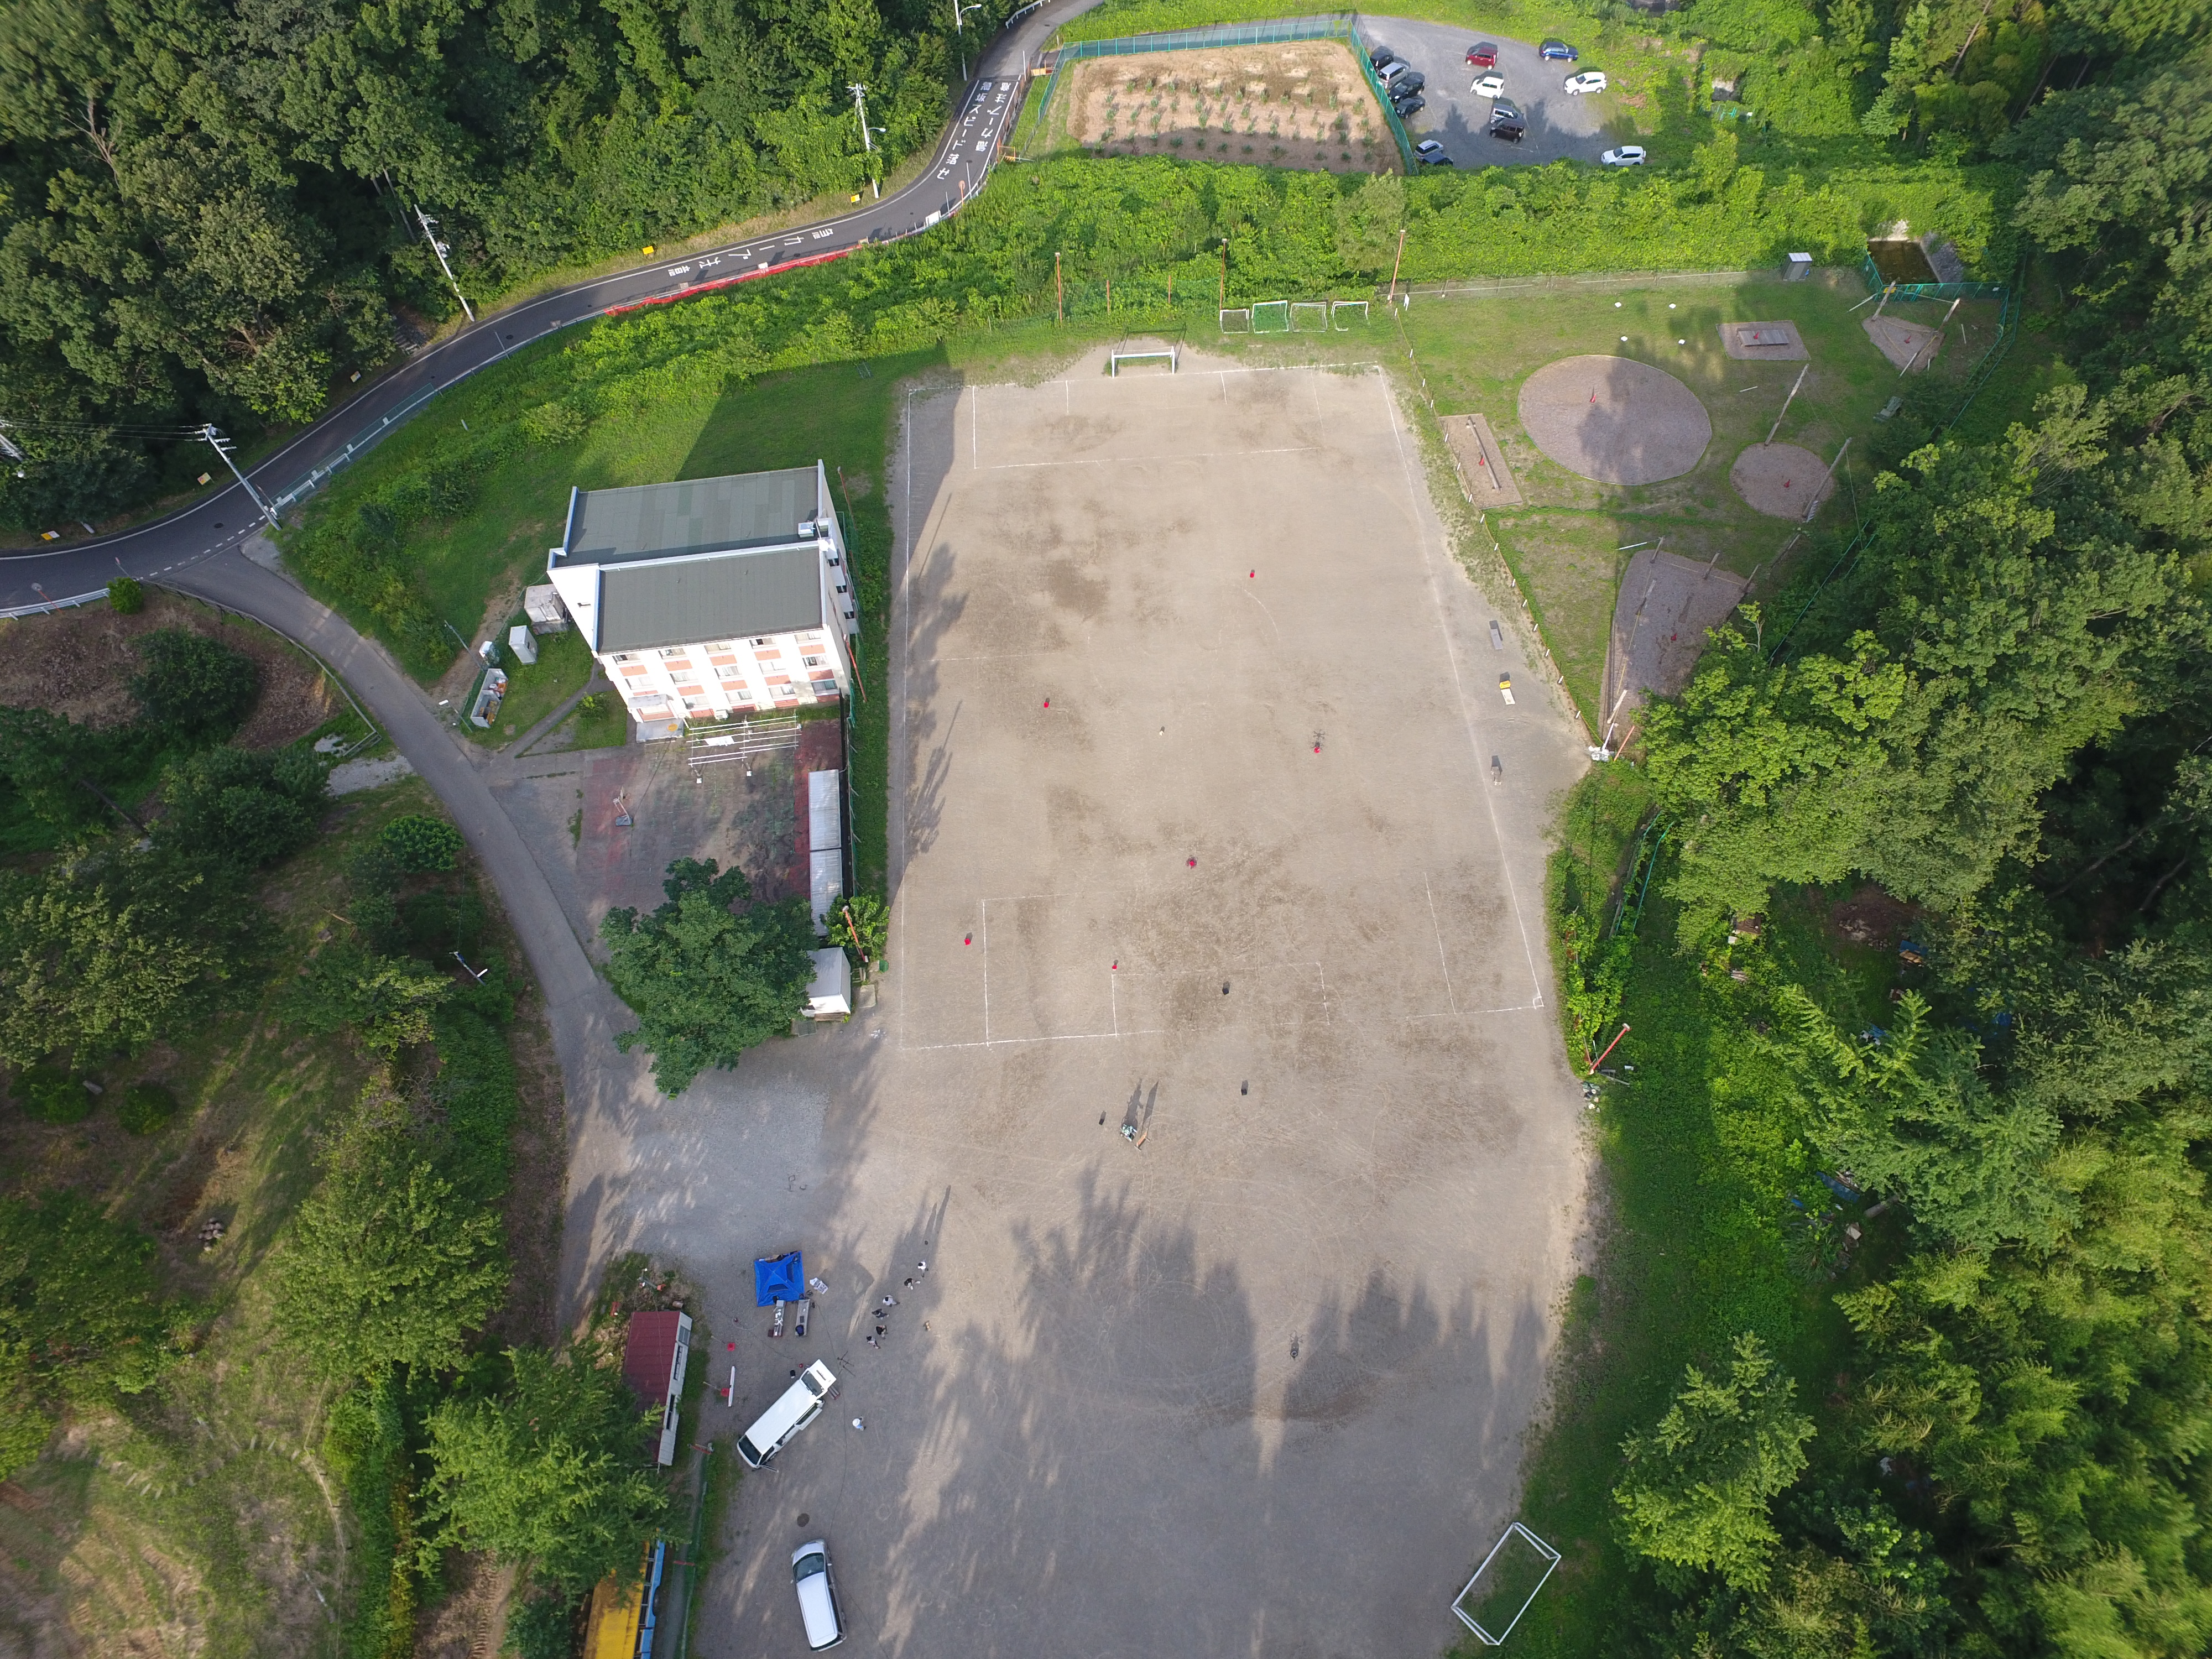
\includegraphics[width=\iwidth, height=\iheight]{sections/grand/images/DJI_0028}}\hspace{1.1em}%
   \subcaptionbox{
     \scriptsize{}\label{fig3:b}}{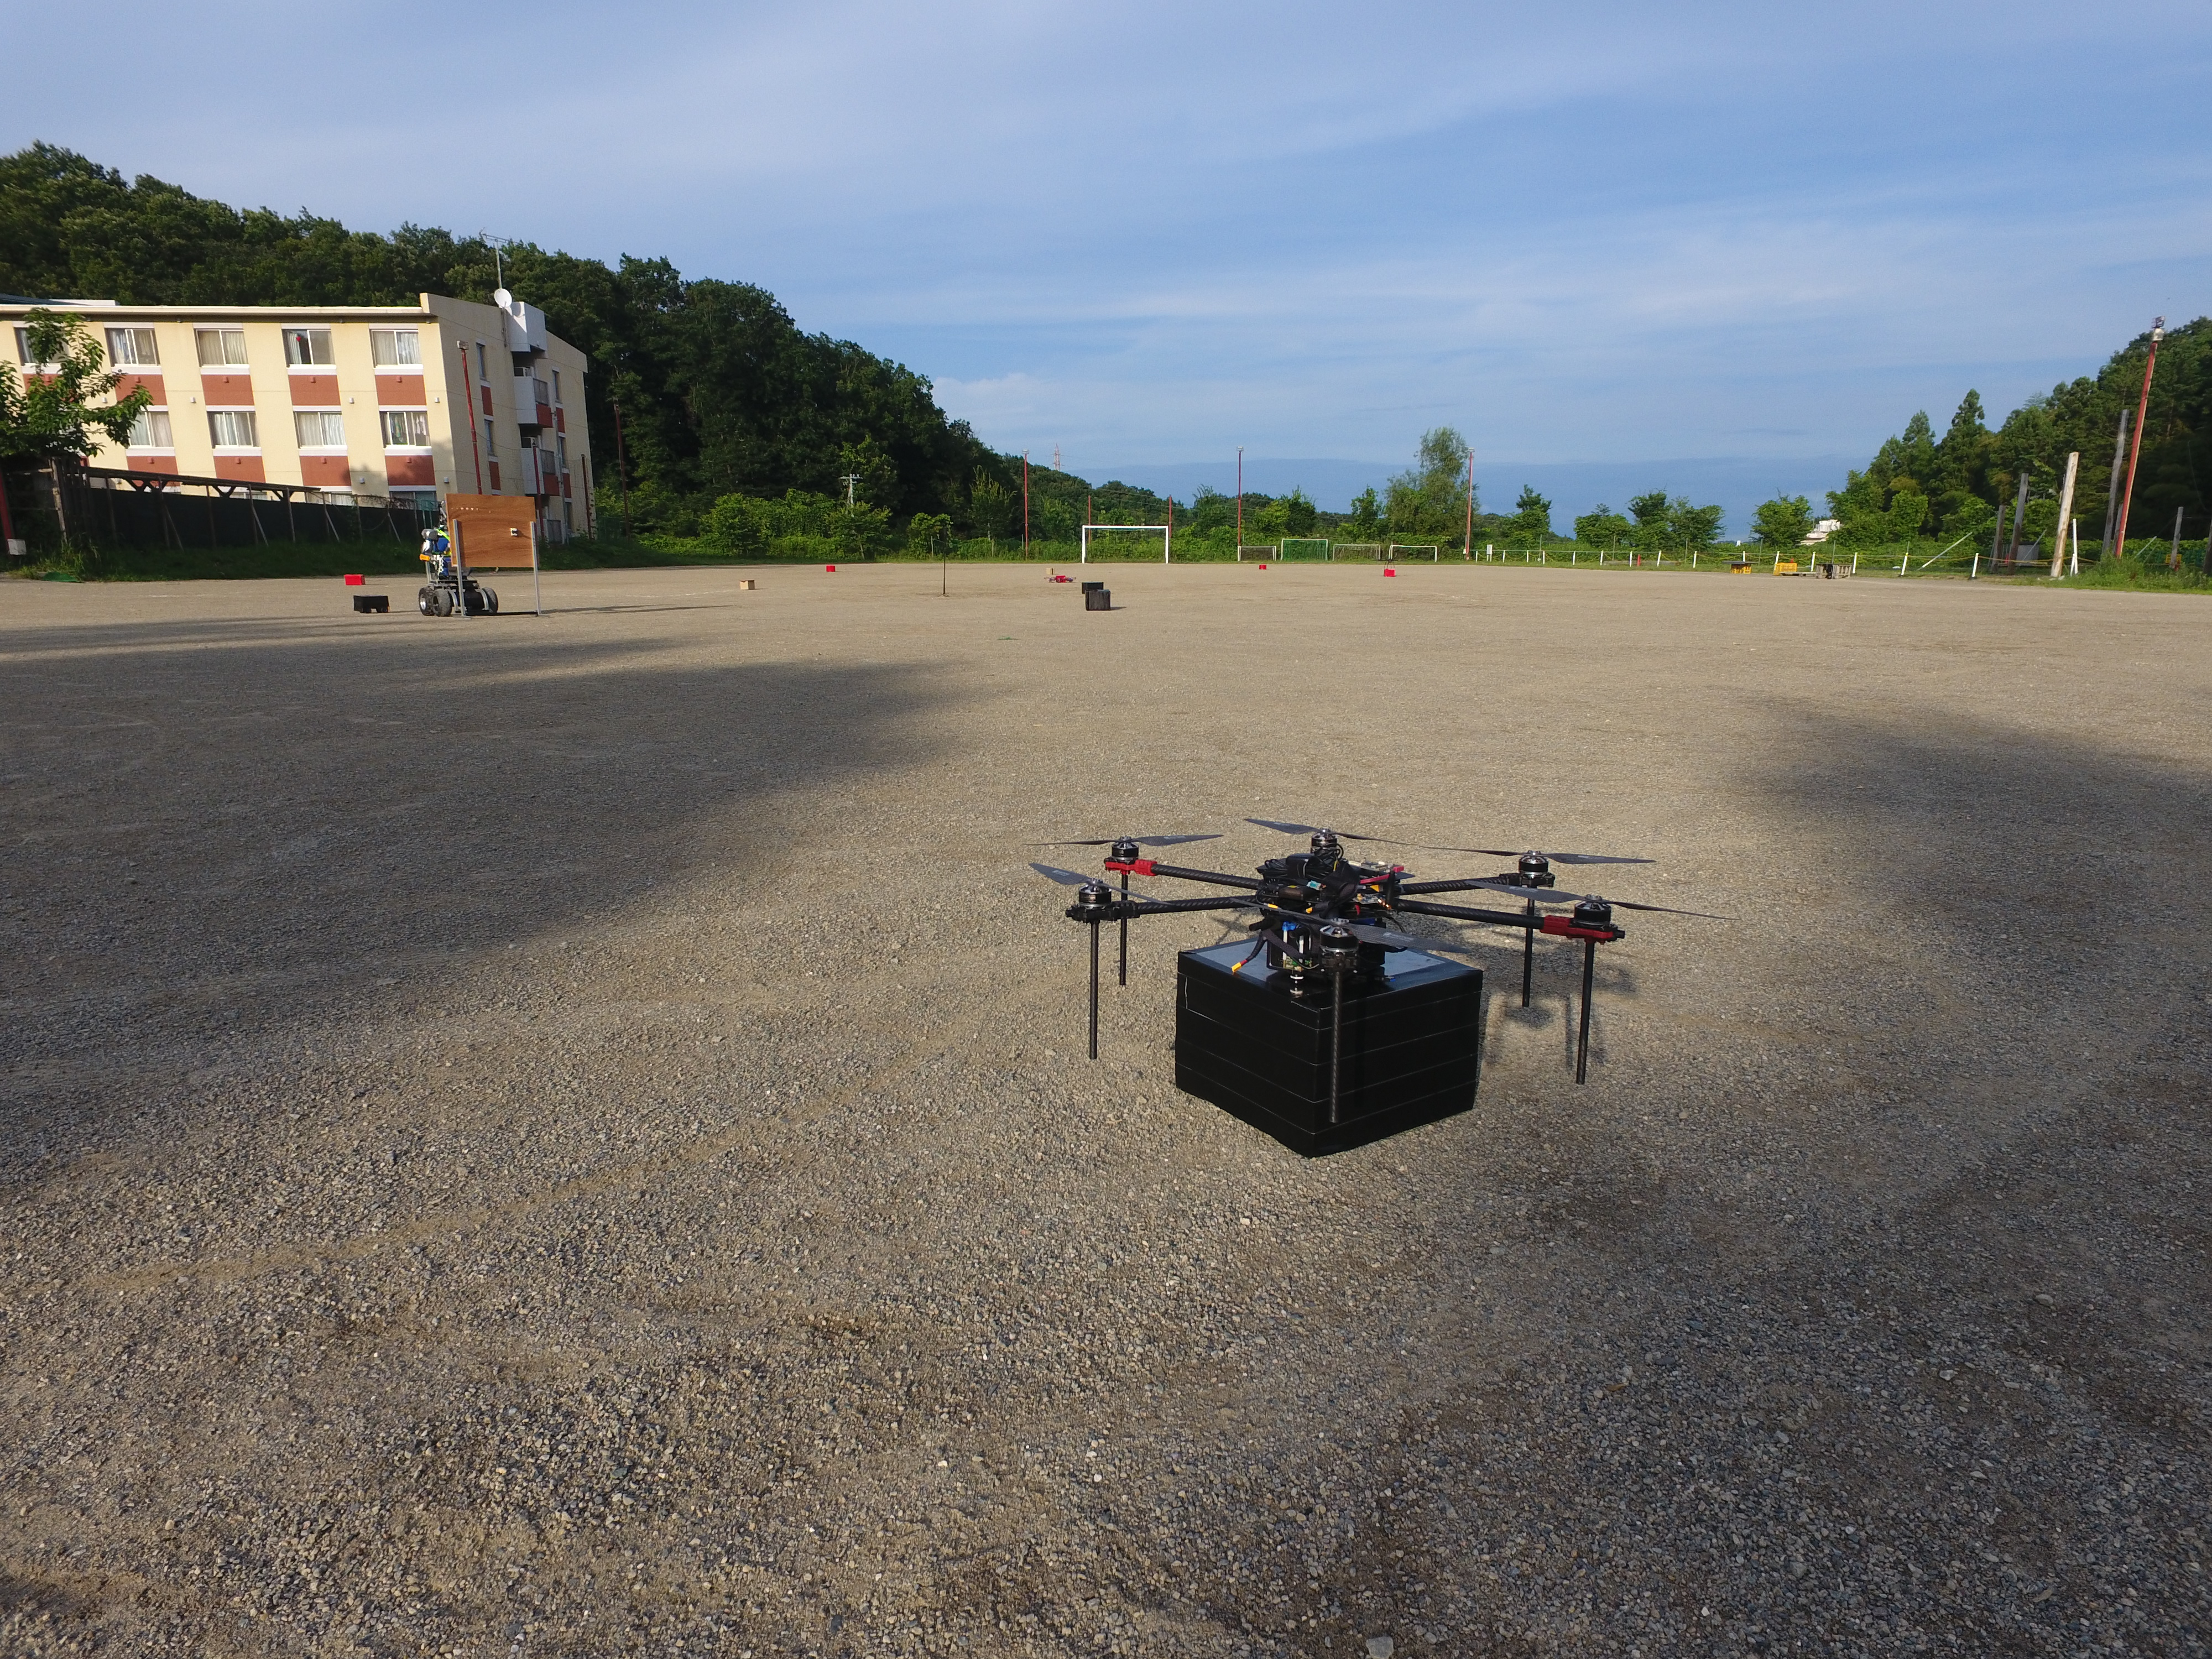
\includegraphics[width=\iwidth, height=\iheight]{sections/grand/images/DJI_0059}}\hspace{1.1em}%
   \subcaptionbox{
     \scriptsize{}\label{fig3:c}}{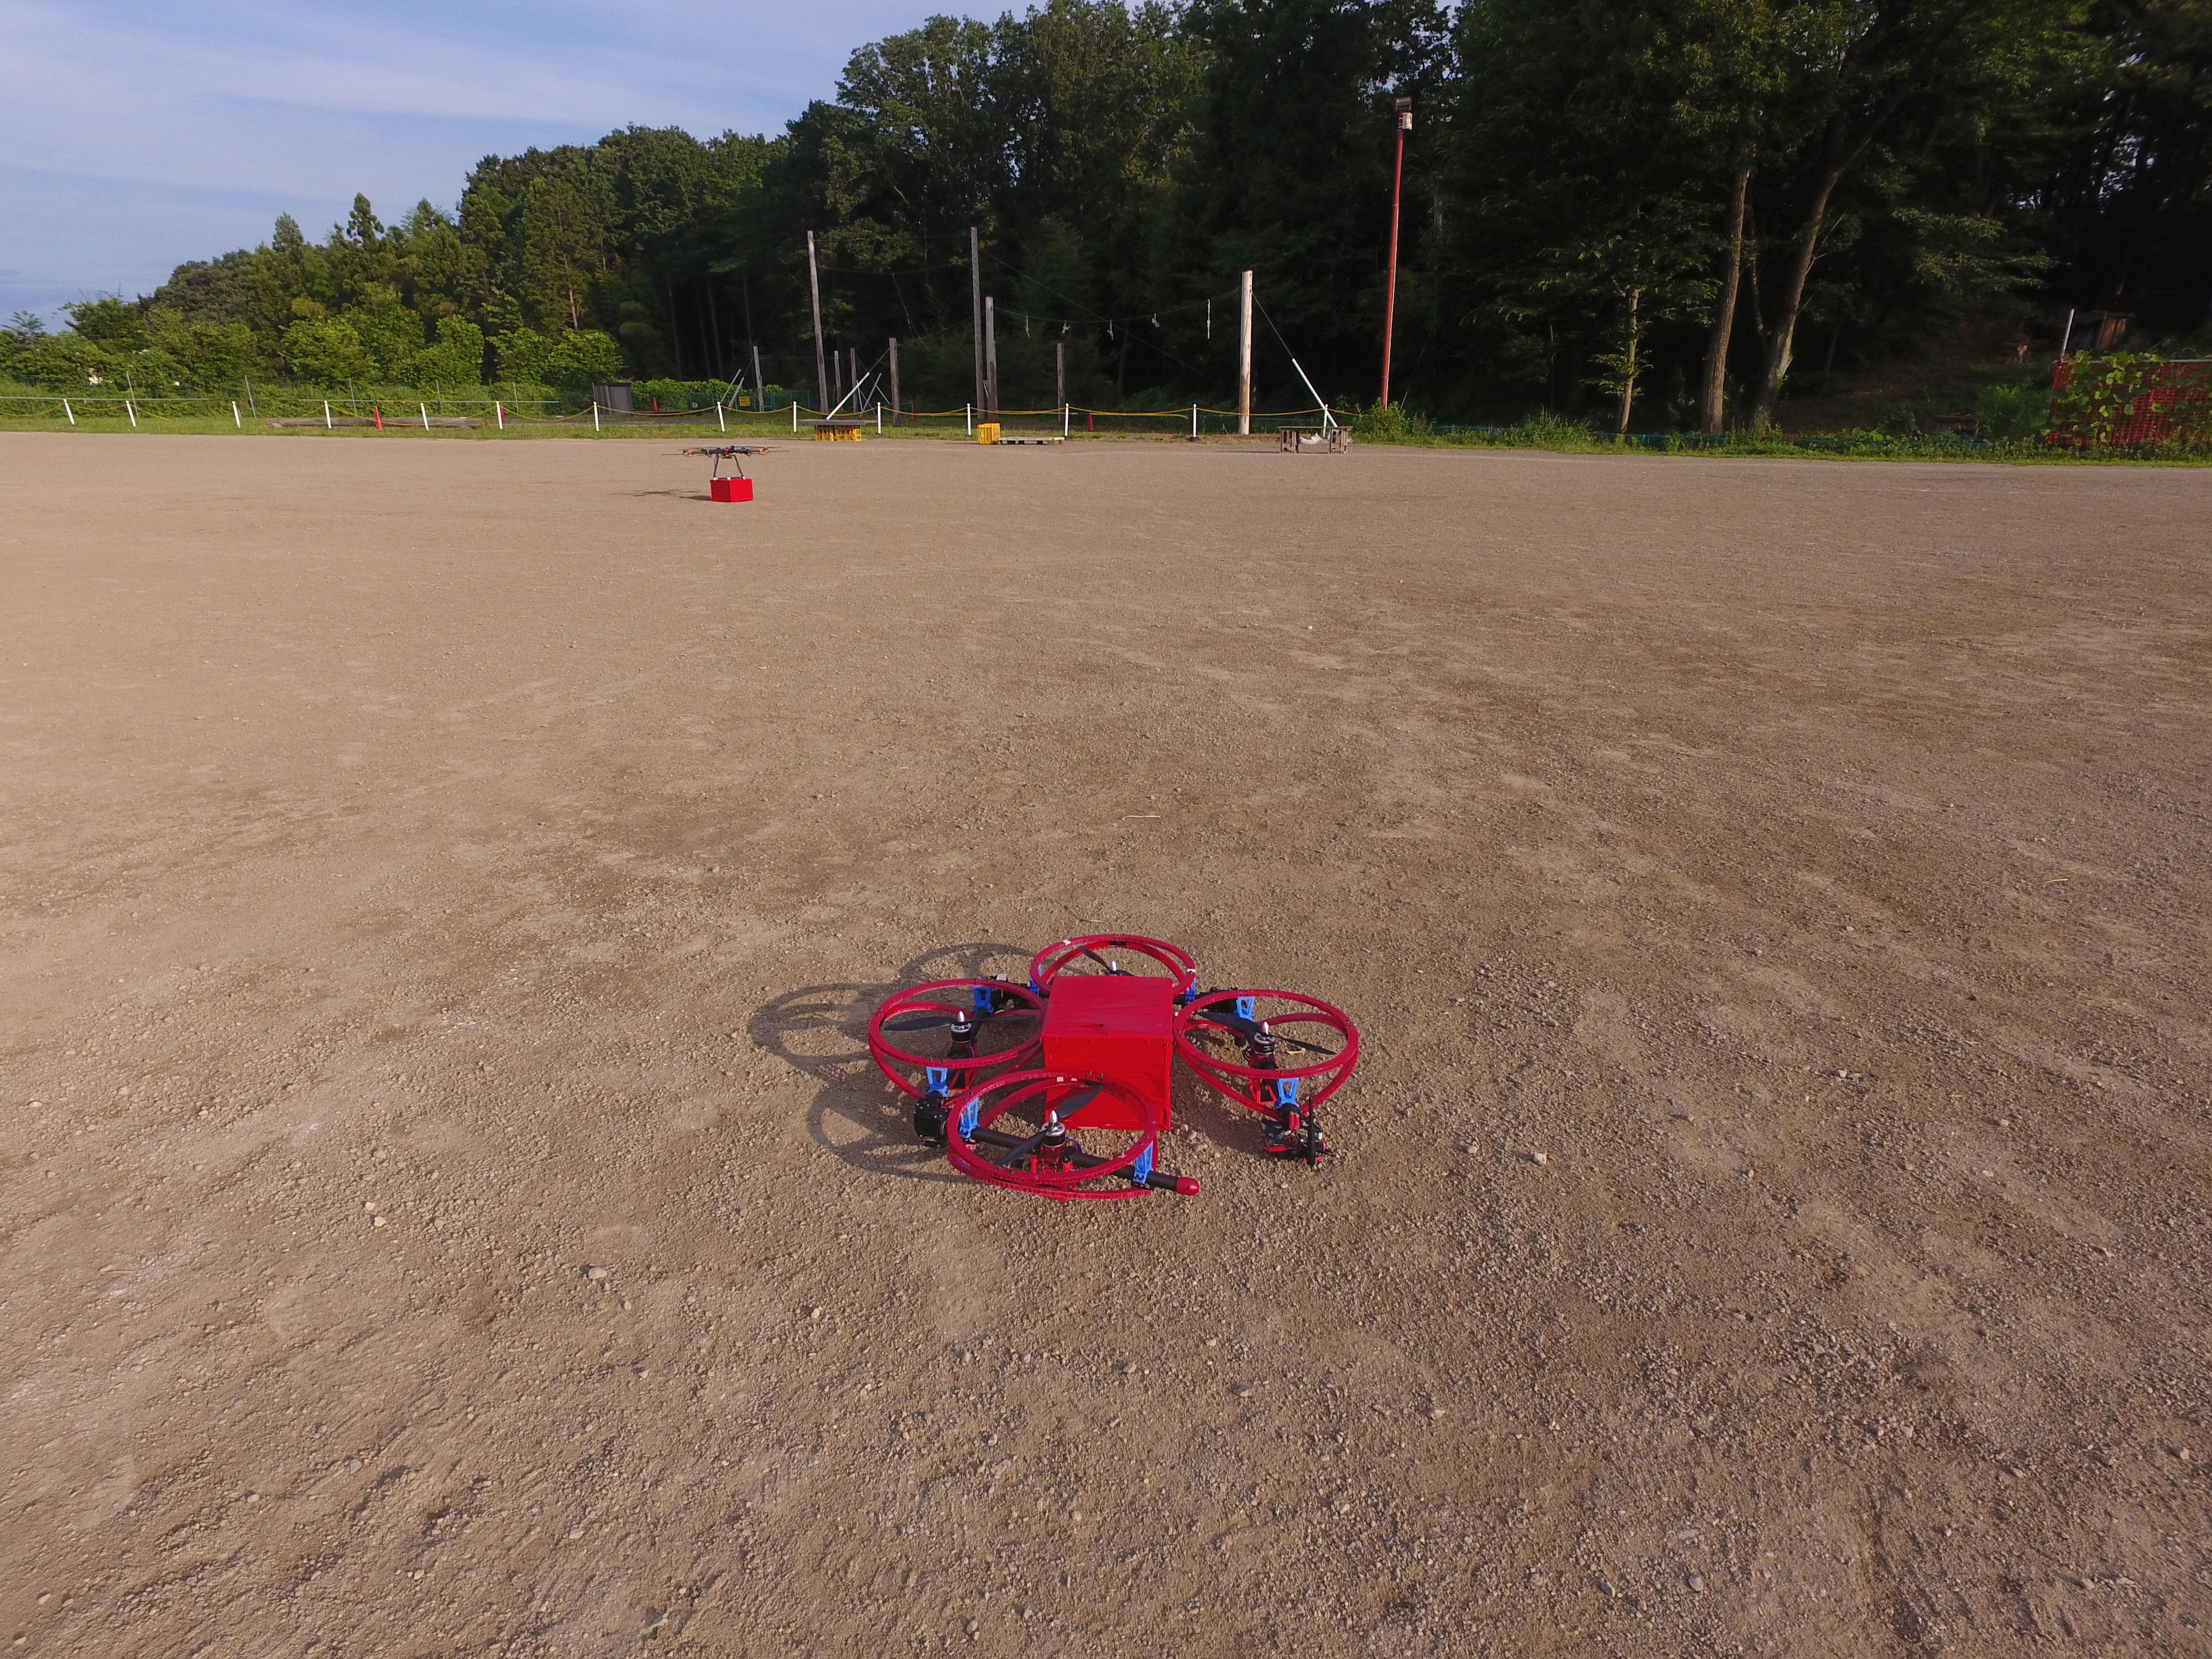
\includegraphics[width=\iwidth, height=\iheight]{sections/grand/images/DJI_0079}}\hspace{1.1em}%
   \subcaptionbox{
     \scriptsize{}\label{fig3:d}}{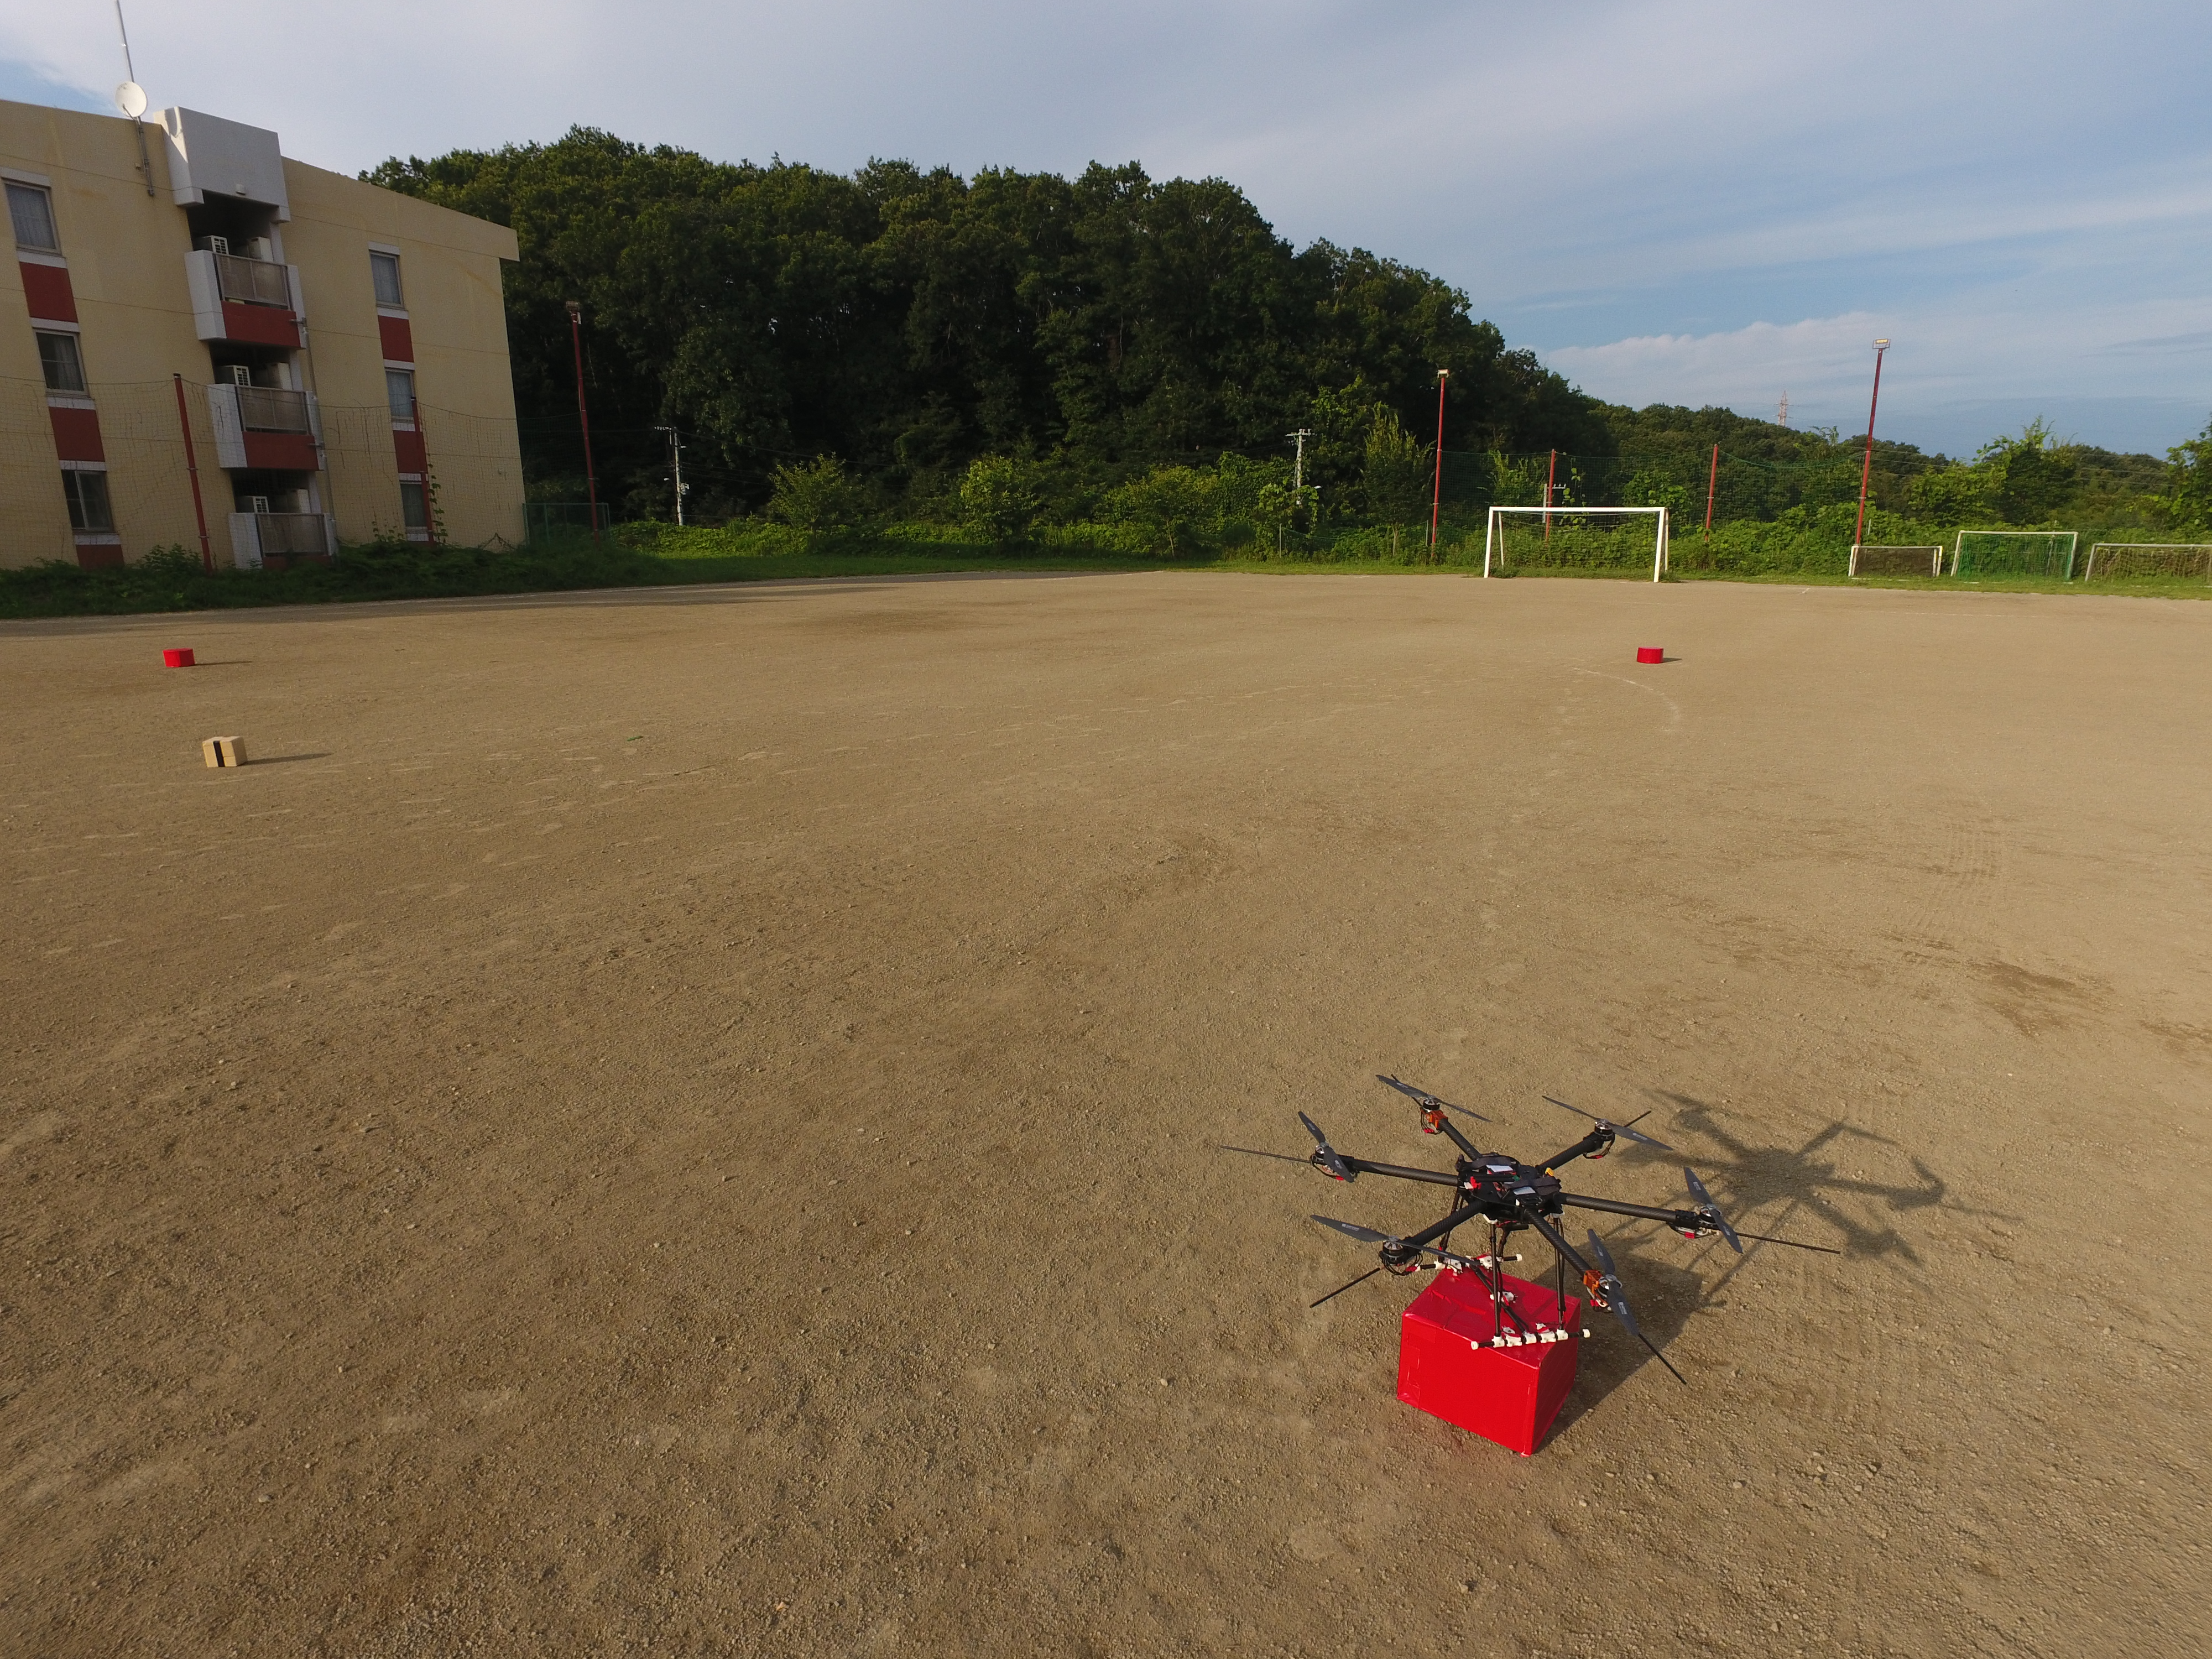
\includegraphics[width=\iwidth, height=\iheight]{sections/grand/images/DJI_0092}}\hspace{1.1em}%
   \caption{JSK--Team testbed setup at Hachioji, Tokyo, Japan}
   \label{fig:objects}
 \end{figure}


\end{document}
